%%%%%%%%%%%%%%%%%%%%%%%%%%%%%%%%%%%%%%%%%%%%%%%%%%%%%%%%%%%%%%%%%
%  _____       ______   ____									%
% |_   _|     |  ____|/ ____|  Institute of Embedded Systems	%
%   | |  _ __ | |__  | (___    Wireless Group					%
%   | | | '_ \|  __|  \___ \   Zuercher Hochschule Winterthur	%
%  _| |_| | | | |____ ____) |  (University of Applied Sciences)	%
% |_____|_| |_|______|_____/   8401 Winterthur, Switzerland		%
%																%
%%%%%%%%%%%%%%%%%%%%%%%%%%%%%%%%%%%%%%%%%%%%%%%%%%%%%%%%%%%%%%%%%

\chapter{Glitches}\label{chap.glitch}

\section{Glitche in der Digitalen Signalverarbeitung}\label{sect.glitch_def}
In der Digitalen Signalverarbeitung ist glitch ein bekannter Fehler, den William I. Fletscher folgendermassen beschreibt: ''Als \textit{glitch}  wird eine ungewollte, flüchtige ''Signalspitze'' bezeichnet, die Zähler aufwärts zählt, Register löscht oder einen ungewollten Prozess startet.'' \cite{F_glitches} \\


Abbildung \ref{fig.glitch.def} zeigt zwei \textit{glitches} in einem Ausgangssignal.\\

\begin{figure}[H]
	\centering
	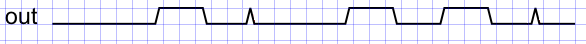
\includegraphics[width=\textwidth]{images/glitch/def_glitch_1.png}
	\caption{Zwei Glitches im Ausgangssignal}
	\label{fig.glitch.def}
\end{figure}


\section{Ursache für Glitches}\label{sect.glitch_ursache}
Der Auslöser sind ungleichzeitig eintreffende Signale, die durch \\
1.) unterschiedlich lange Signalpfade, \\
2.) unterschiedliche Durchlaufverzögerungen der vorangehenden Flip-Flops oder \\
3.) unterschiedliche Logik-Zeiten \\
entstehen, und die in ein asynchrones Bauteil geführt werden.\\
Der Dekoder im asynchronen Bauteil entschlüsselt dadurch kurzfristig einen falschen Wert. \\

Abbilung \ref{fig.glitch.bild1} zeigt ein leicht verzögertes (getaktetes) enable-Signal zu einem anders verzögerten (getakteten) Flip-Flop-Eingangssignal Q. Der Ausgang des Flip-Flops weist kurzzeitig Glitches auf. \\
\begin{figure}[H]
	\centering
	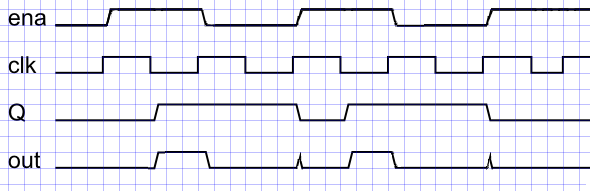
\includegraphics[width=0.8\textwidth]{images/glitch/def_glitch_3.png}
	\caption{Asynchrone Eingangssignale führen zu Glitches}
	\label{fig.glitch.bild1}
\end{figure}


\newpage
\section{Glitches durch Pfadverzögerung erzeugen}\label{sect.glitch_detect}
Die Pfade eines asynchronen Dekoders werden durch Routing verlängert.

\subsubsection{Konzept}
Dekodiert wird die Zahl 15. Durch intelligentes Routing (FF 1 wird verzögert, FF 2 wird beschleunigt) wird der Zustand der Zahl 11 forcier 

\subsubsection{Implementation} 
Cyclone II, Board De2. Quartus 13.0sp.

Die Pfad\textit{verlängerung} wird über das Routing über die GPIO-Pins des Headers 1 gemacht (siehe Abbildung \ref{fig.glitch.routing}. Die obersten vier Doppel-Pins erhalten eine "Brücke", sodass das Signal links ausgegeben und rechts wieder eingespiesen wird.\\
Signal\textit{verkürzung} ist eine direkte Signalzuweisung \todo {korrektes Wort ?(Concourent Assignment)} .\\
\begin{figure}[H]
	\centering
	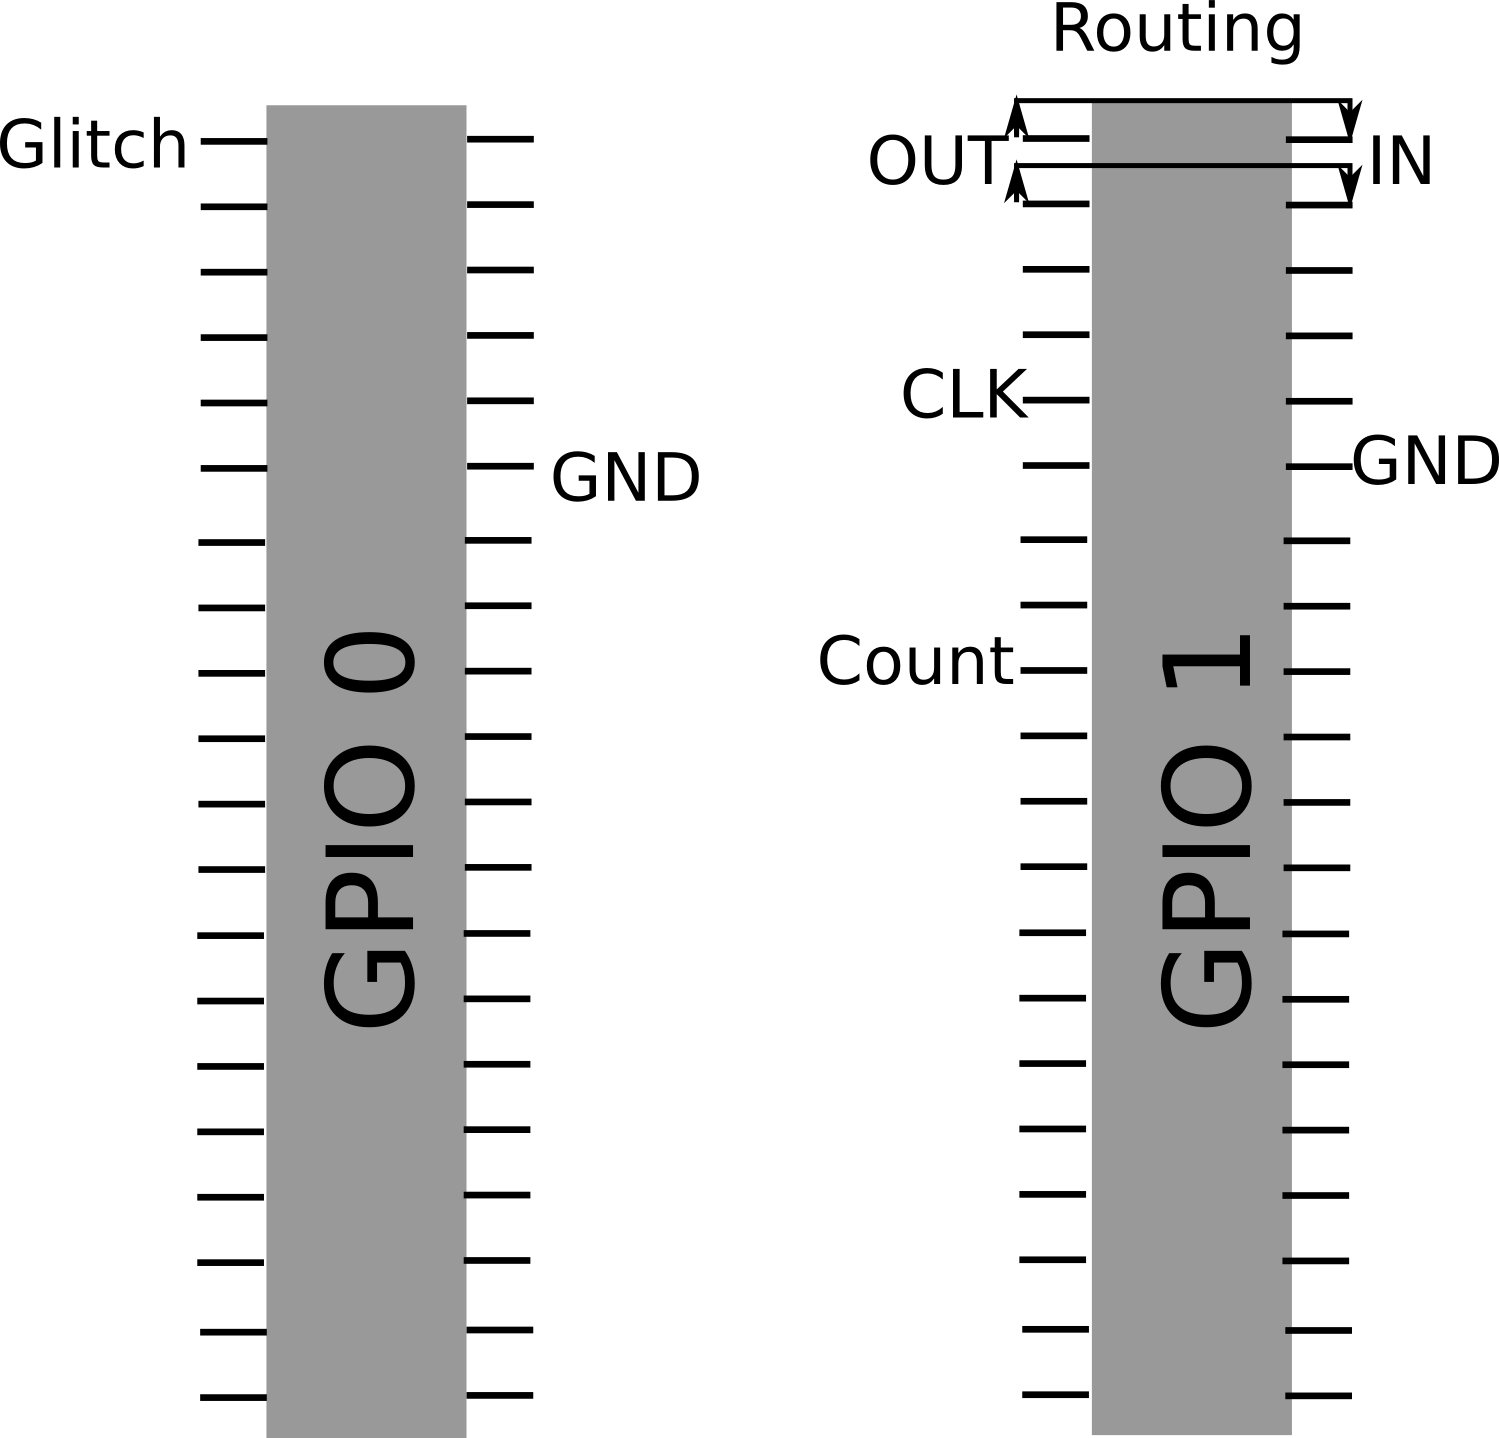
\includegraphics[width=0.3\textwidth]{images/glitch/GPIO_Belegung.png}
	\caption{GPIO Anschlüsse}
	\label{fig.glitch.GPIO}
\end{figure}

Auf dem KO wird das asynchrone Glitch-Signal und das synchrone Zählersignal neben dem Takt ausgegeben. Weil der Zähler synchronisiert wurde, ist der Wert 1 Periode (= 20 ns) später als der Glitch.\\

\begin{figure}[H]
	\centering
	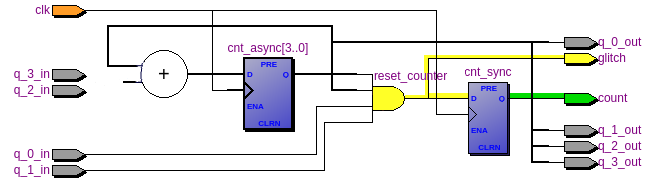
\includegraphics[width=\textwidth]{images/glitch/RTL_glitch_detection_bemalt.png}
	\caption{Zähler mit Signal-Routing über GPIO}
	\label{fig.glitch.routing}
\end{figure}
Im RTL-Diagramm sieht man deutlich den Unterschied zwischen dem asynchronen Zähler, der über das Gate \textit{reset\_{counter}} beim Wert 15 einen Impuls an den Ausgang glitch gibt und dem synchronisierten Zähler \textit{cnt\_{sync}} der dem asynchronen Ausgang nachgeschaltet ist und dieses Signal taktet. Das getaktete Zähl-Signal geht an den Ausgang \textit{count}.


	
\section{Resultat Glitches provozieren}\label{sect.glitch_resultat}

\subsection{Erzeugen über Bauteiltoleranzen}
Der Ansatz, dass die Bauteiltoleranzen der Flip-flops eine Ursache für asynchrone Inputs in den Dekoder sind ist korrekt. Die Umsetzung zeigte sich jedoch als schwierig, da die heutigen Flip-Flops zu schnell sind bzw. ihre Toleranzen zu klein um sichtbar zu werden. \todo {Timeanalyse für FF} Aus diesem Grund entschlüsselte der asynchrone Dekoder trotz kleinen Verzögerungen die Werte stets korrekt.\\



\subsection{Erzeugen über Routing} 
\begin{figure}[H]
	\centering
	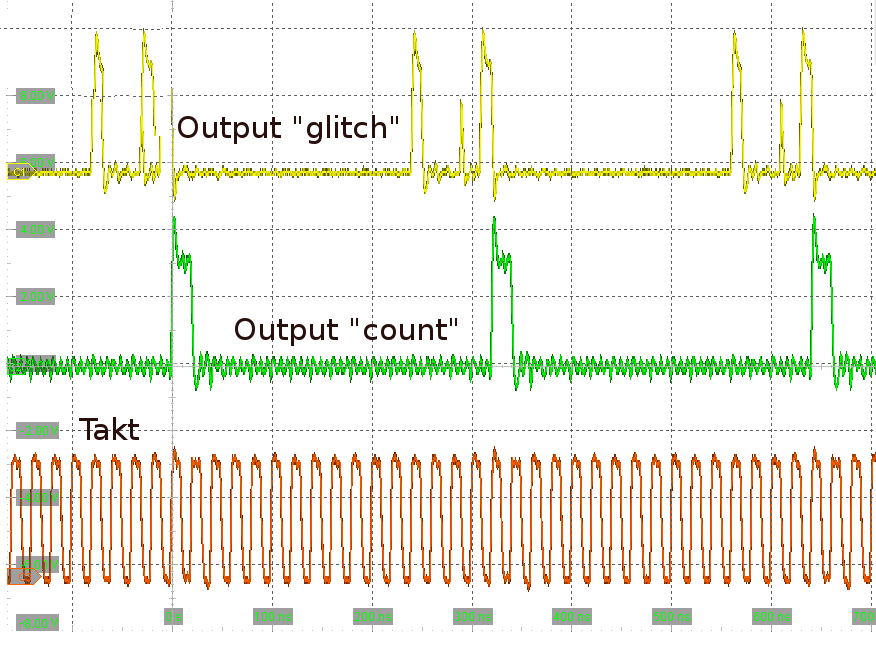
\includegraphics[width=0.8\textwidth]{images/glitch/Glitch_2_good_kommentar.png}
	\caption{Glitch (gelb), Zähler (grün) und Takt (orange)}
	\label{fig.glitch.result_1}
\end{figure}

Typisch ist, dass der synchrone Zähler eine Signalbreite von genau einer Periode hat, da dieses Signal getaktet ist. Dagegen hat der asynchrone Glitch keine konstante Breite.
\begin{enumerate}
	\item{Bei welchen Zählständen treten Glitches auf?}

	\item{Wie hängen die Zählständen mit dem gewählten Routing zusammen?}

\end{enumerate}
